\chapter{実装}
%ラズパイマウスのfollowerノードについての実装を書く.今はspheroとラズパイマウスのwiibordを本実装として話しているため改変が必要.aproachに持っていく.
\begin{figure}[ht]
    \centering
    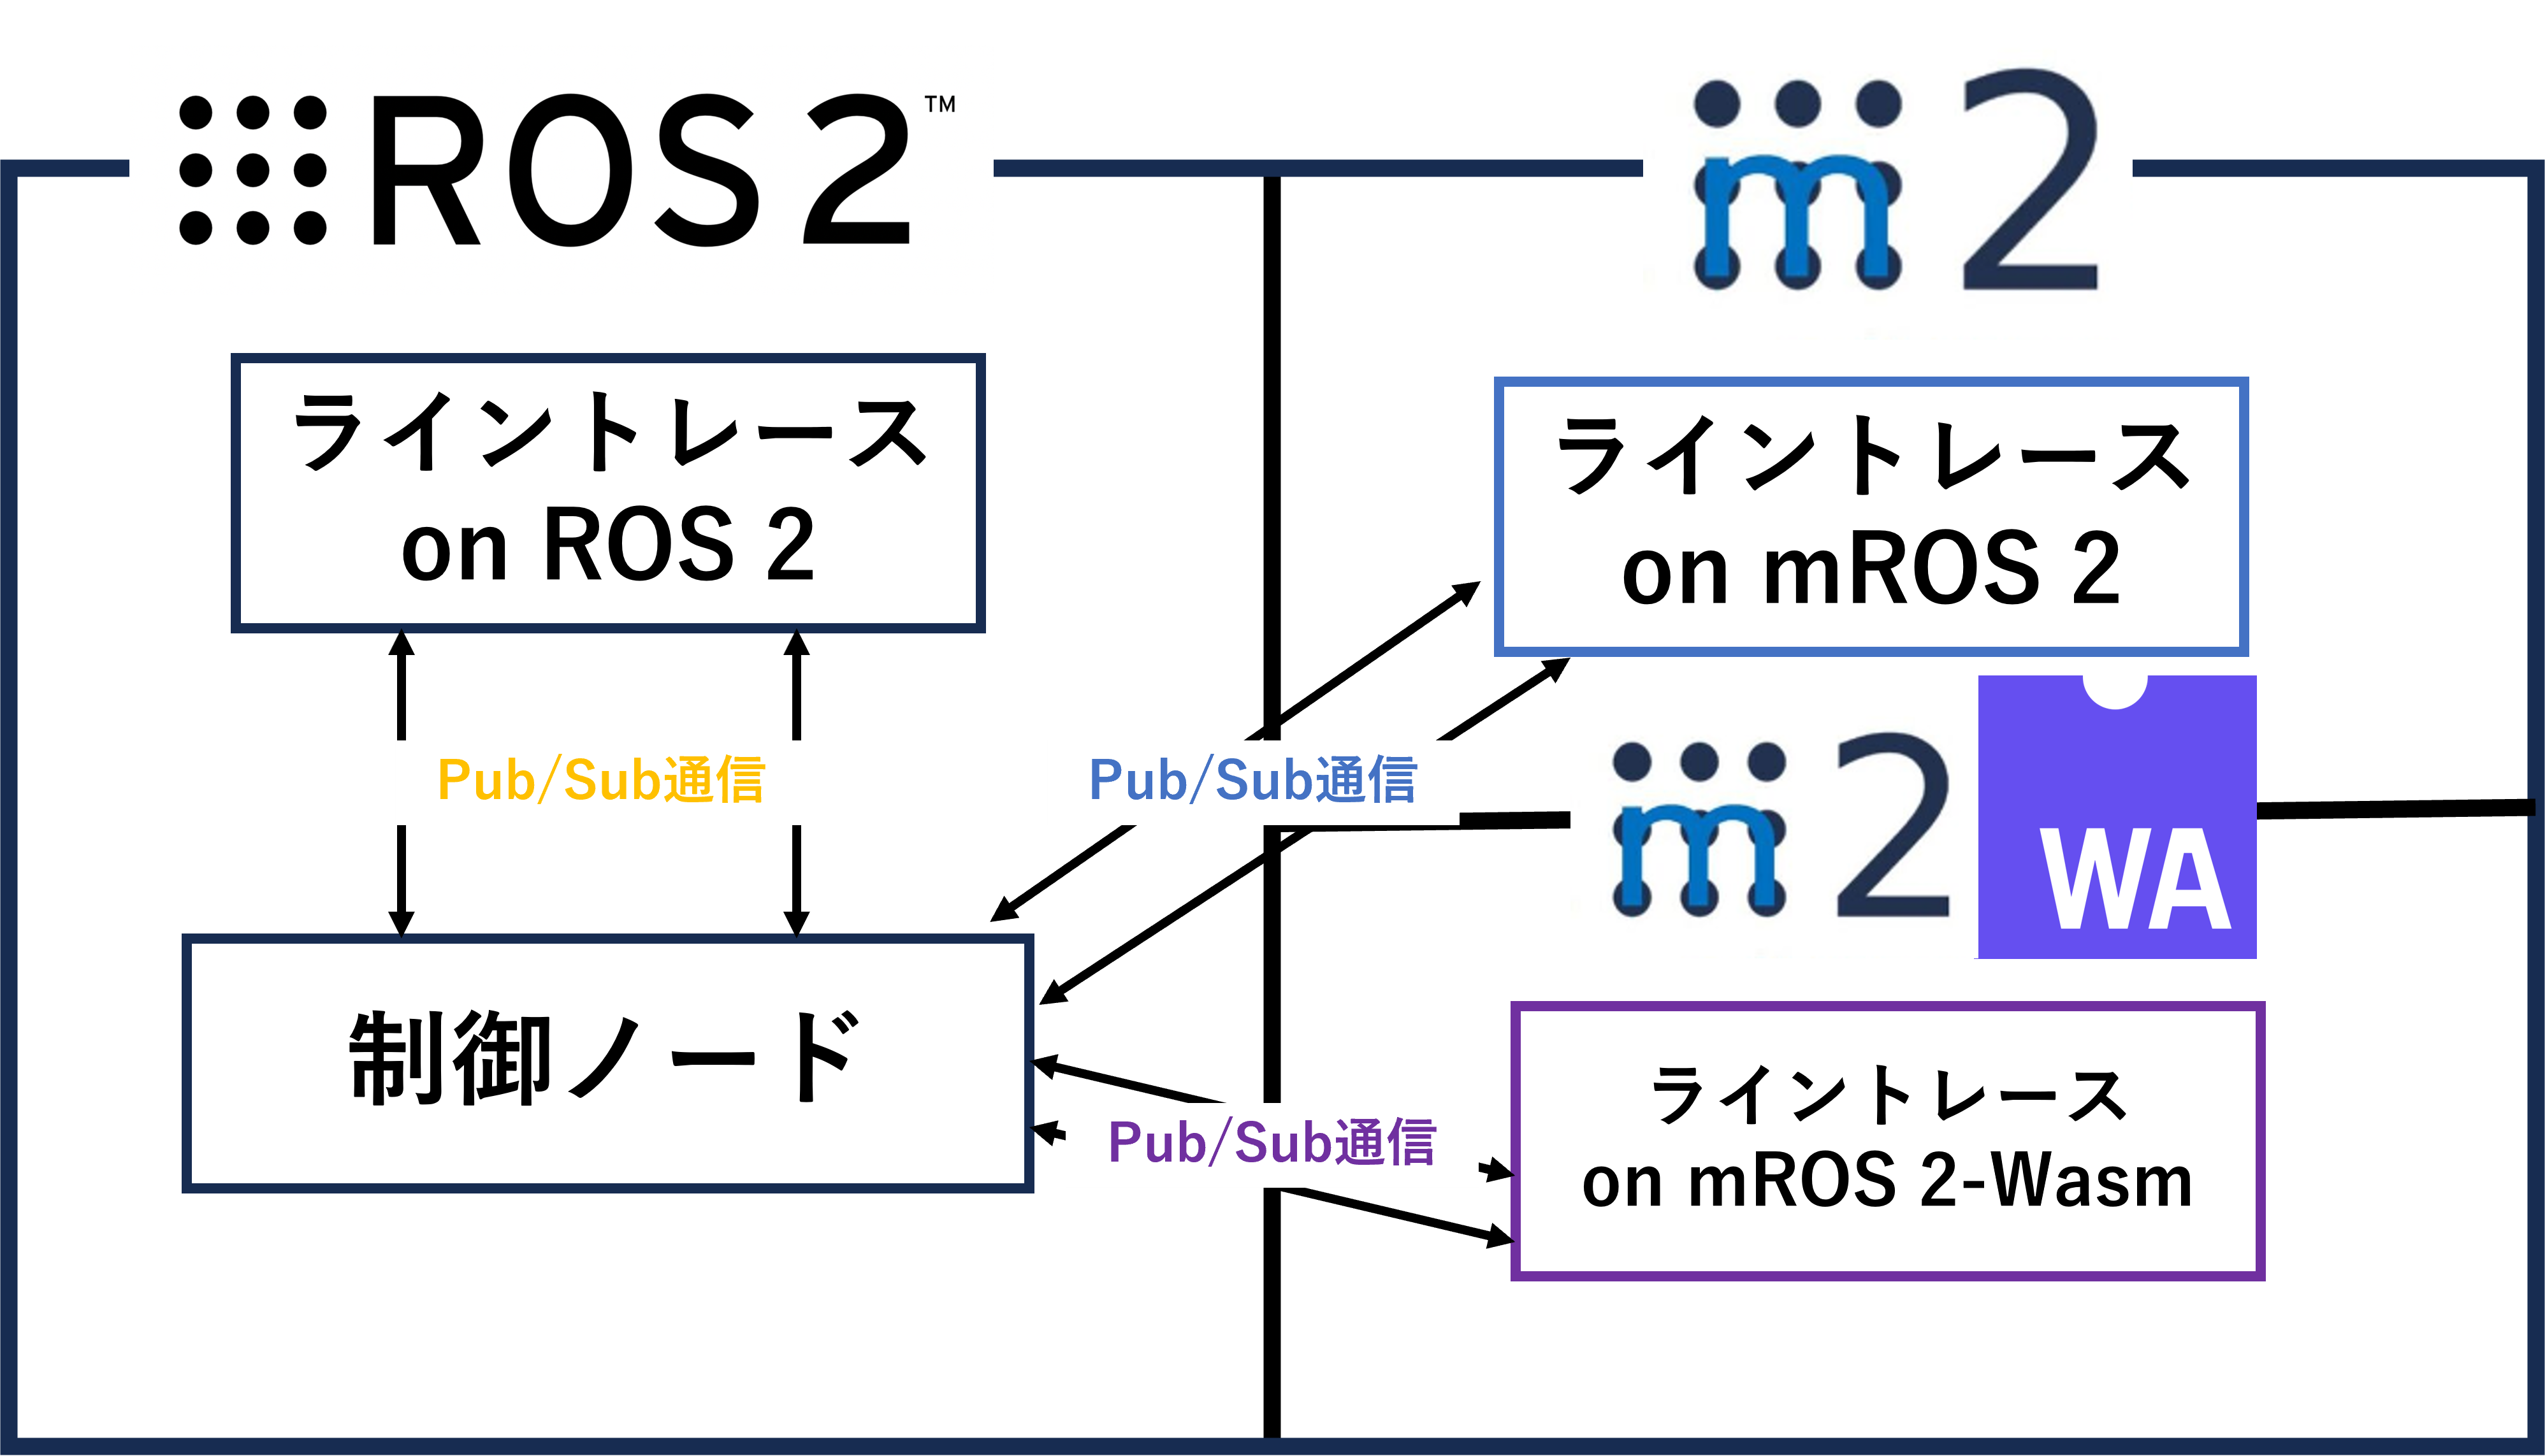
\includegraphics[width=15cm]{images/fig4_mros2_ros2_raspimouse_configuration.png}
    \caption{実装アプリケーション構成}
    \label{fig:mros2_ros2_raspimouse_configuration}
\end{figure}
\begin{figure}[h]
    \centering
    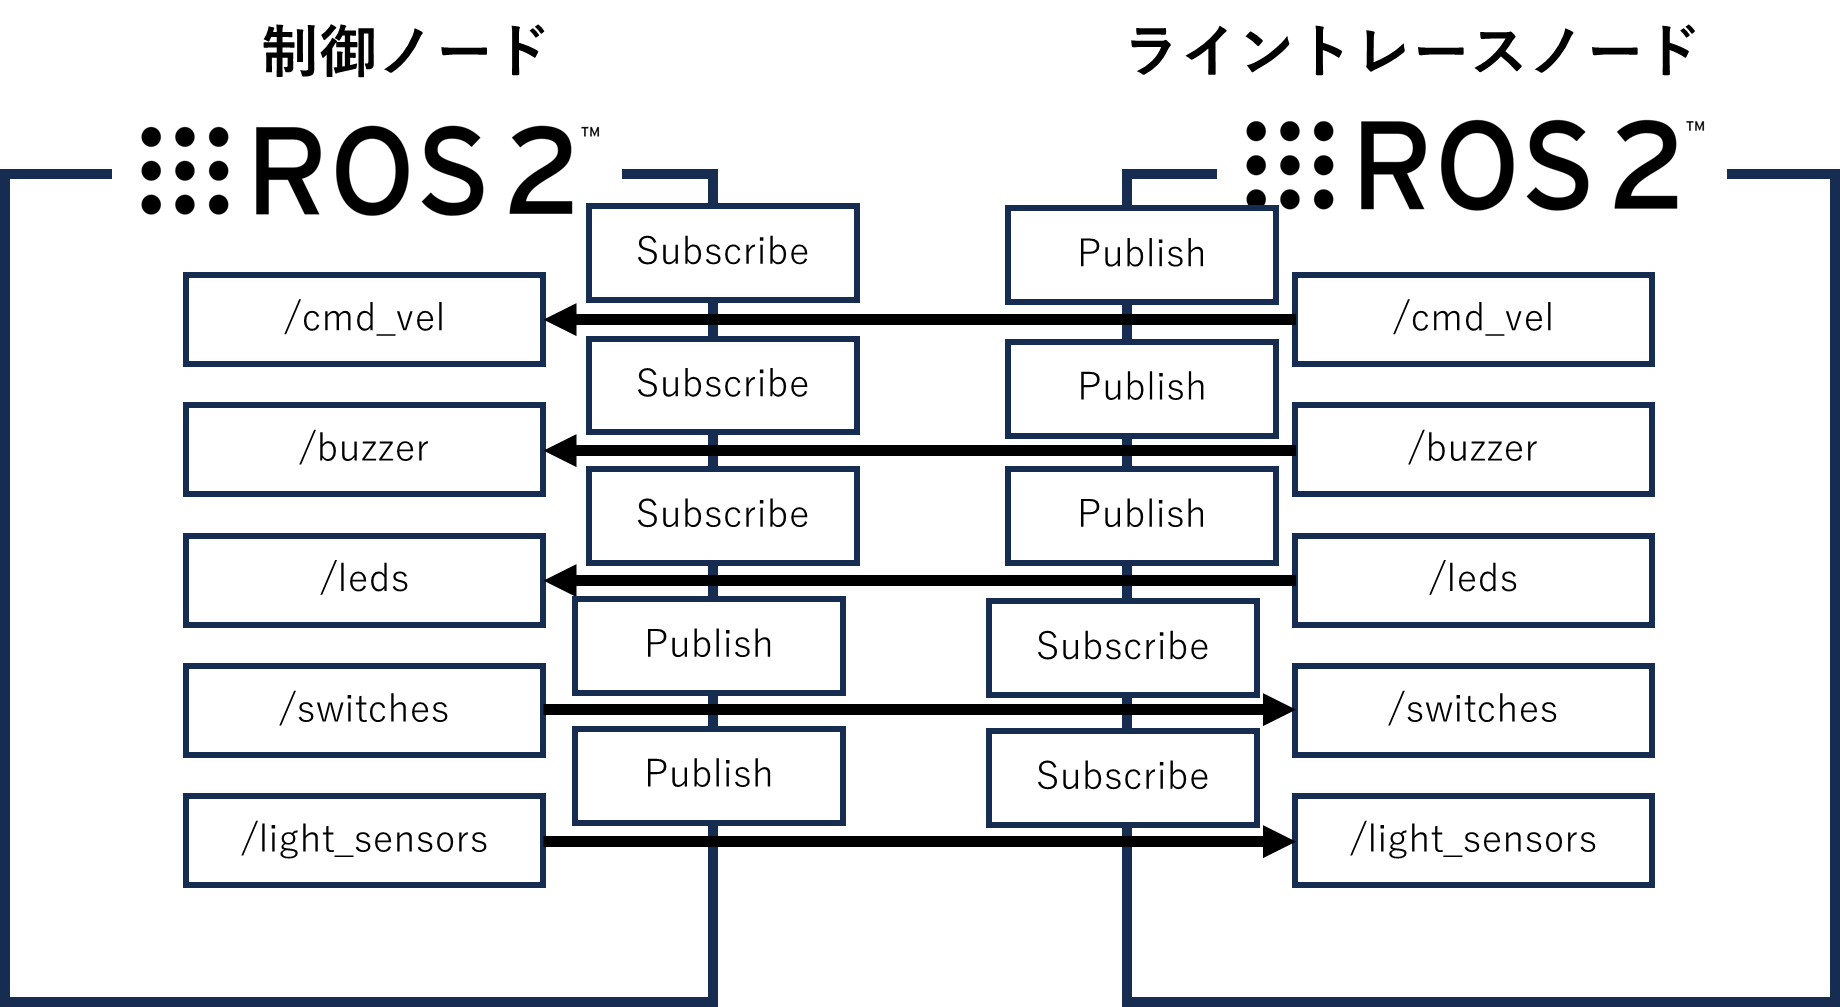
\includegraphics[width=15cm]{images/fig4_pubsub_configuration.png}
    \caption{実装アプリケーションのPub/Sub通信構成}
    \label{fig:mros2_ros2_pubsub_configuration}
\end{figure}

\begin{figure}[h]
    \centering
    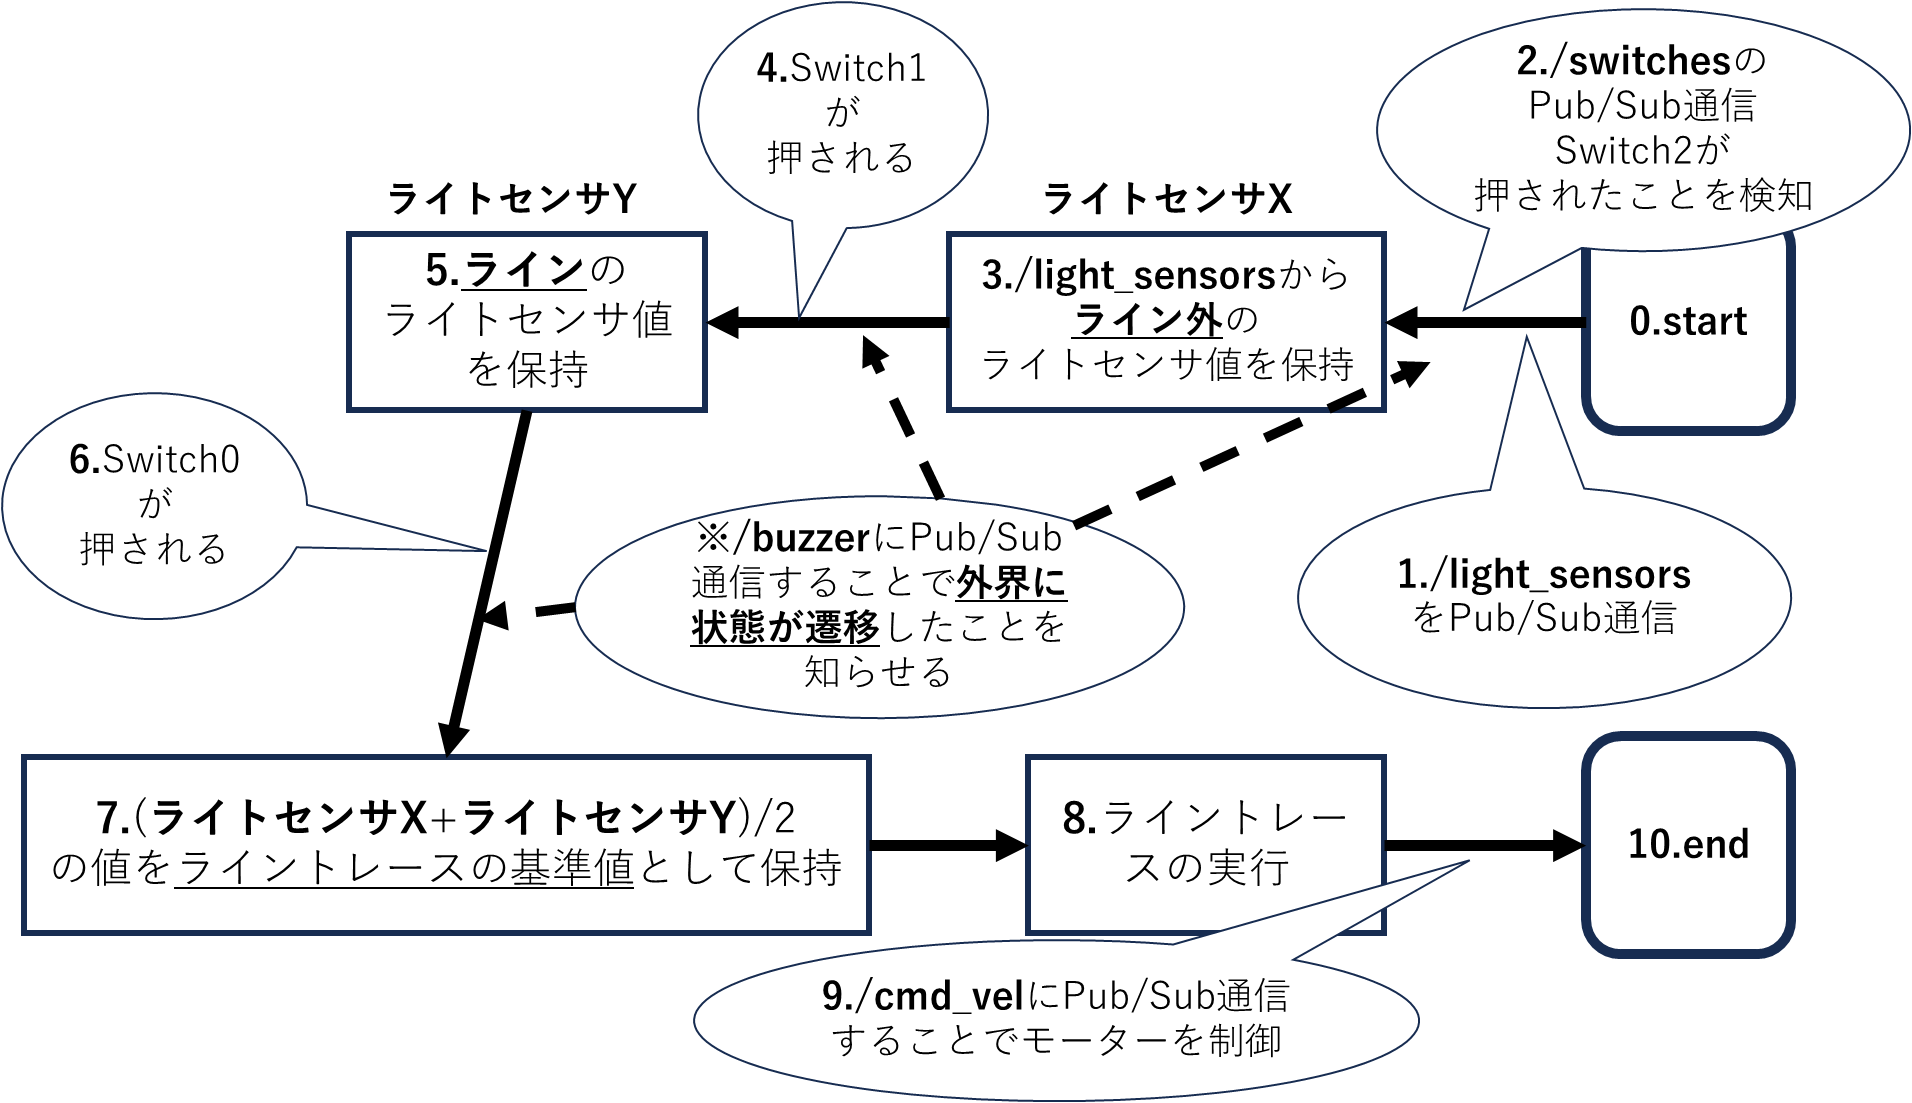
\includegraphics[width=15cm]{images/fig5_moveflow.png}
    \caption{実装アプリケーションの動作フロー}
    \label{fig:moveflow}
\end{figure}

\begin{figure}[h]
    \centering
    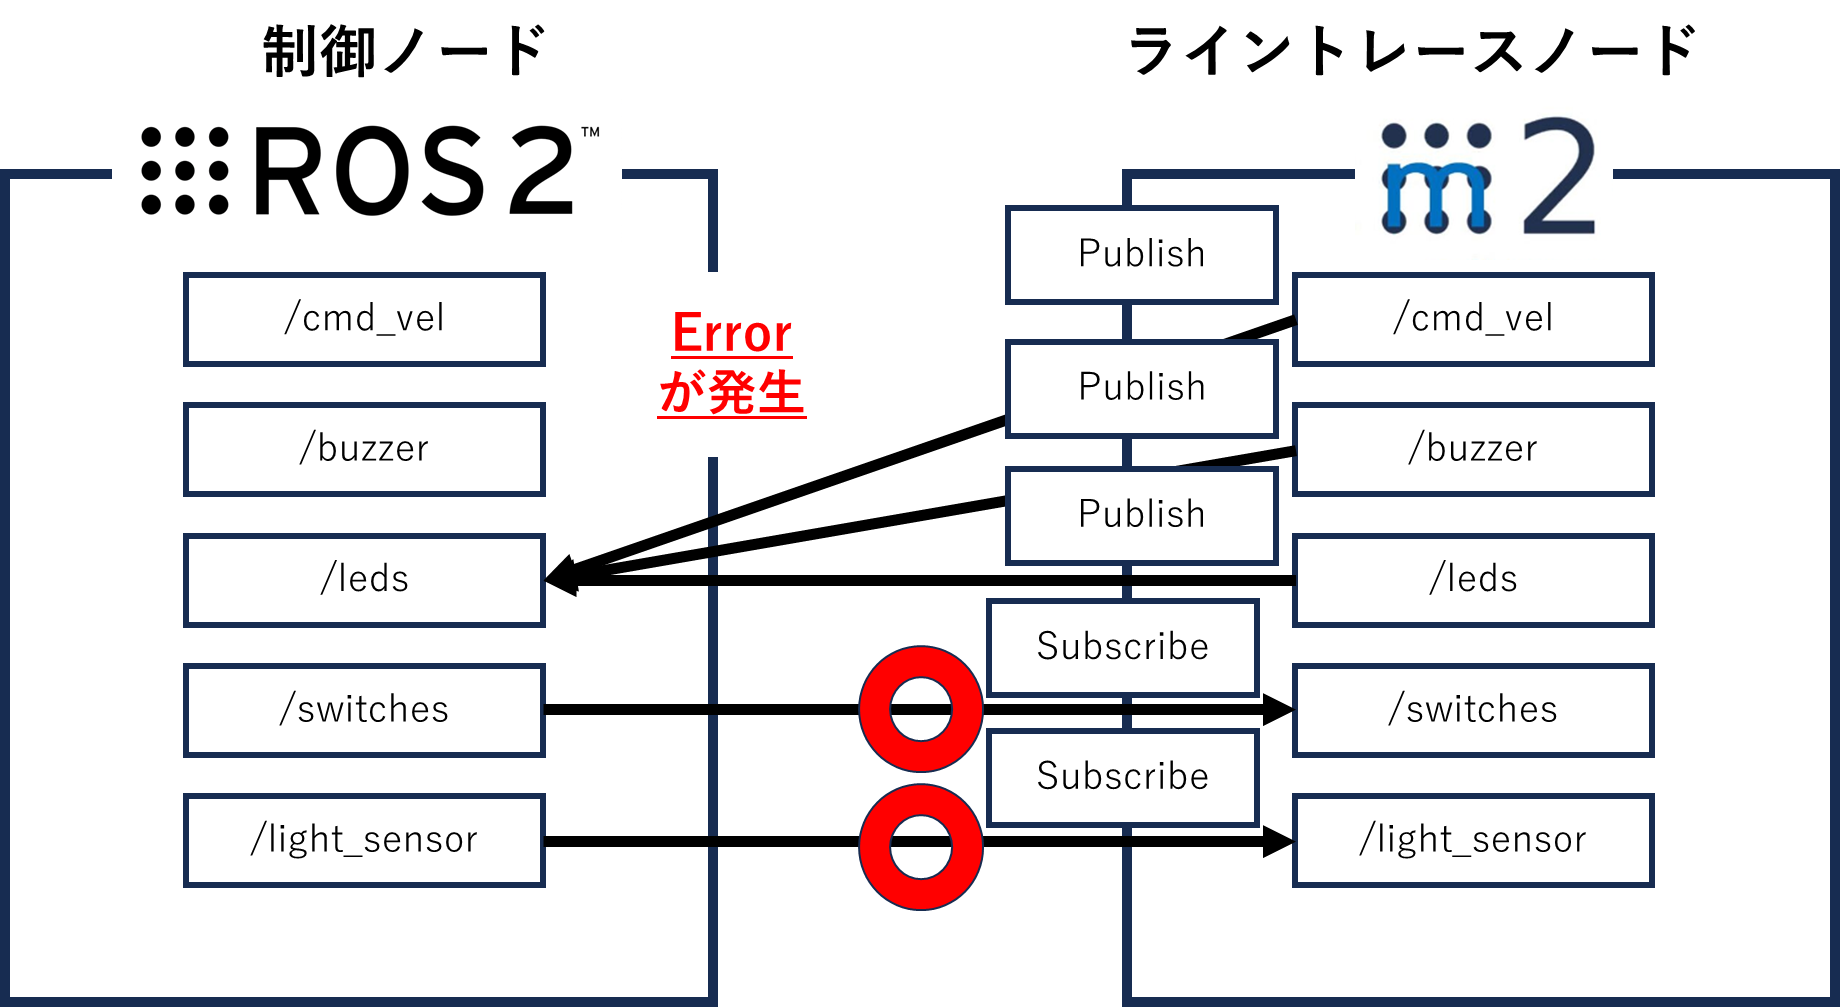
\includegraphics[width=15cm]{images/fig4_mros2bug.png}
    \caption{mROS 2-POSIXのバグ}
    \label{fig:mros2bug}
\end{figure}

\begin{figure}[h]
    \centering
    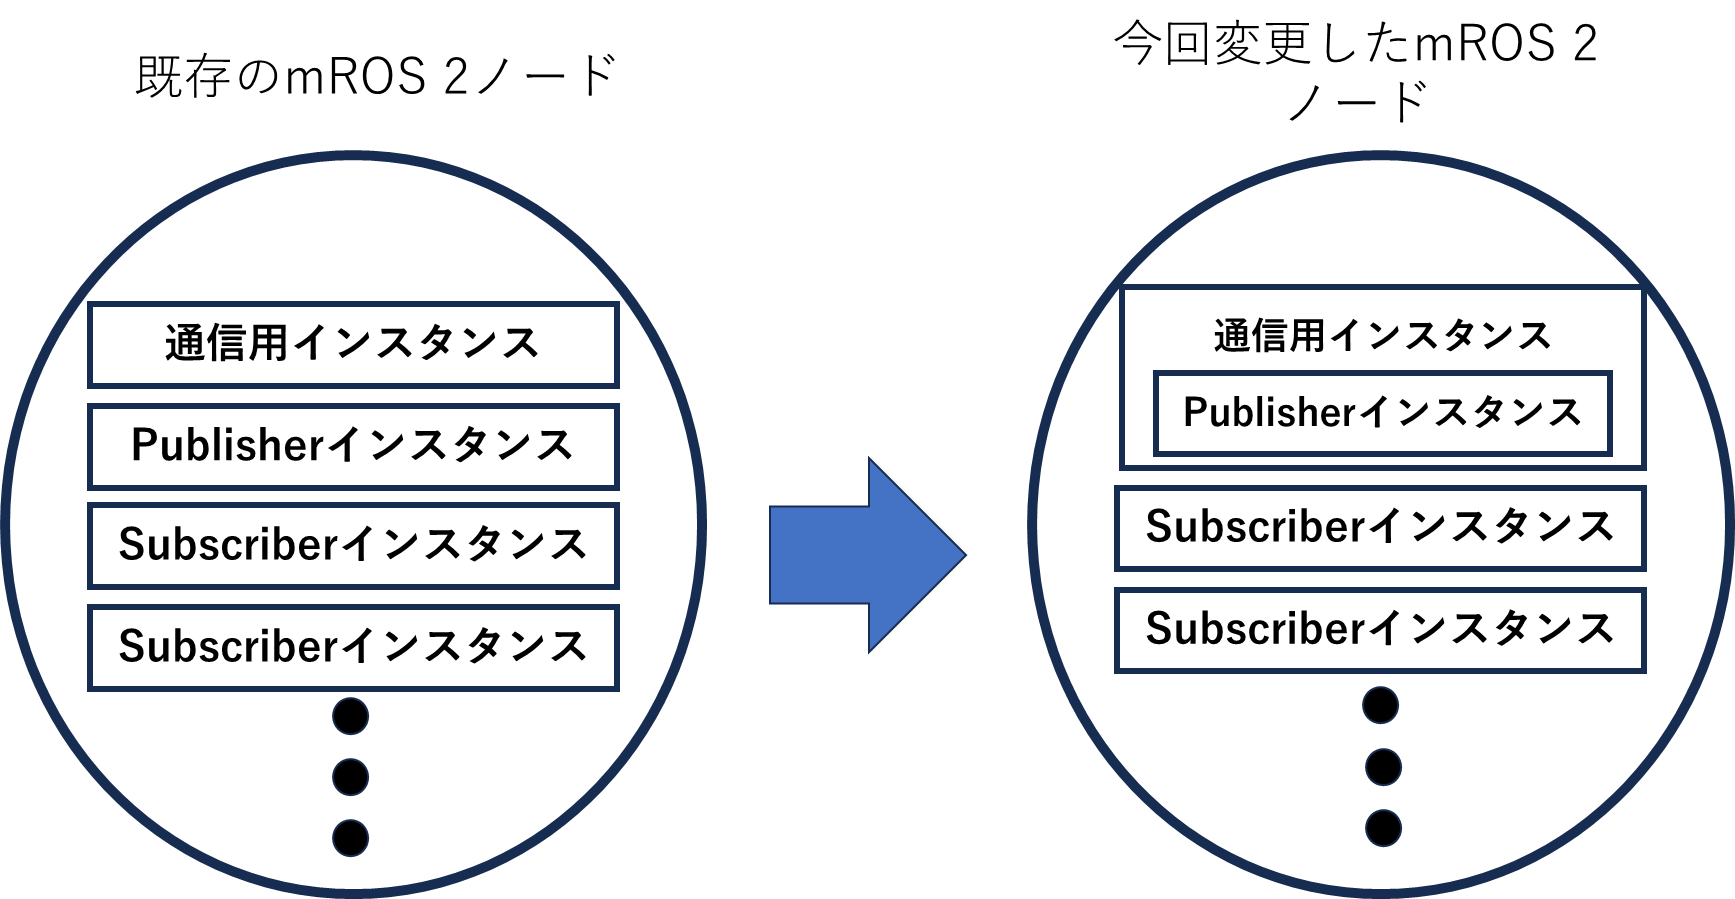
\includegraphics[width=15cm]{images/fig4_mros2bug_fix.png}
    \caption{mROS 2-POSIXのバグ fix}
    \label{fig:mros2bug-fix}
\end{figure}
\label{chap:implementation}
%書くこと
%ラズパイマウスのfollowerノードについての実装

\noindent 本章では,mROS 2-POSIXとROS 2の性能を比較評価するにあたって,実装するアプリケーションの概要について説明する.
\section{実装要件}
mROS 2-POSIXとmROS 2-WasmとROS 2を比較評価するためのアプローチとしてROS 2で実際に動作するアプリケーションが望ましい.
第1章で述べた通り,mROS 2-POSIXの評価はネットワークスループットのマイクロベンチマークに留まり,実アプリケーションにおける有用性が十分に評価されていない.
そのため,mROS 2-POSIXとmROS 2-WasmとROS 2に以下の条件を満たしたアプリケーションを実装し,比較評価を行う.
実装するアプリケーションの要件として,Pub-Sub通信を主な機能として使用しているアプリケーションであること,組み込みデバイス上で動作できるアプリケーションであること,OSへの依存が少ないアプリケーションであることの3つを要件とした.
まず,ROS 2にはPub/Sub通信やService通信,Action通信があるが,mROS 2-POSIXとmROS 2-POSIXを基盤としたmROS 2-Wasmには,Pub/Sub通信のみの実装になっている.
これはmROS 2-POSIXで使用されているembeddedRTPSが組込み向けの通信プロトコルであり,軽量化を図るためPub/Sub通信のみの実装になっているからである.
そのため,ROS 2のアプリケーションをmROS 2-POSIXとmROS 2-Wasmに移植する際には,Pub/Sub通信を主な通信手段としているアプリケーションが望ましい.
\\ 次に,本研究は第1章で述べた通り,動的配置機構実現後のロボットソフトウェア基盤としてどのような優位性があるのか明らかにすることを目指している.
したがって,実装するアプリケーションは動的配置機構が適用されるRassberry PiやJettson nanoのような組込みデバイス上で動作できるアプリケーションが望ましい.
\\ 最後に,第1章で述べた動的配置機構は,OSへの依存が少ないアプリケーションが望ましい.
これは,OSの環境に依存したアプリケーションであればあるほど,マイグレーション後の環境で正常に動作しない可能性が大きくなるためである.
\\ 以上の条件を満たすアプリケーションとして,本研究ではラズパイマウスで動作するROS 2のライントレースノードをmROS 2-POSIXとmROS 2-Wasmに移植し,比較評価を行う.
\\ ライントレースとは,ロボットや自動車などの自動制御システムが,地面に引かれた線に沿って移動する技術のことである.
主に,教育や趣味,競技の分野で用いられる技術で,センサーを使って線を認識し,それに従って機体を制御する.この実現には,光センサや赤外線センサを使って線の色や反射特性を検出し,そのその情報に基づいてモーターを制御して進路を調整する.主に線が白色で背景が黒,もしくはその逆が一般的である.
\\ このライントレースはロボティクスや自立走行車において基本的な技術であり,将来的により大きなアプリケーションに発展できる可能性がある.
そのため,評価だけでなくmROS 2-POSIXとmROS 2-Wasmのロボットソフトウェア基盤として拡張性示すことができると考え,ラズパイマウスのライントレースノードを各環境に実装することとした.
\section{実装アプリケーションの構成}
本研究ではROS 2で動作するライントレースノードをmROS 2-POSIXに移植し,mROS 2-POSIXとmROS 2-wasm,ROS 2の性能を比較評価する.
比較評価のためのアプリケーションの構成図を図\ref{fig:mros2_ros2_raspimouse_configuration},図\ref{fig:mros2_ros2_pubsub_configuration}に示す.
\\ 図\ref{fig:mros2_ros2_raspimouse_configuration}はmROS 2-POSIXとmROS 2-wasm,ROS 2の実装アプリケーションの構成である.
ラズパイマウスのライントレースアプリケーションは,実際にラズパイマウスを制御する制御ノードと,ライントレースの実装ノードの2つに分かれている.
制御ノードはラズパイマウスのデバイスファイルにアクセスし,モータを回転させたり,LEDやSwitch,ライトセンサの値を取得する.
ライントレースノードは,制御ノードから受け取ったLED,Switch,ライトセンサの値を駆使してモータ制御の命令を制御ノードに向けて通信する.
そのため,制御ノードはOSの依存が大きく,ライントレースノードはOSの依存が少ない.
前述の通り,マイグレーションはOS依存があるアプリケーションに適用すると,適用後に動作しない可能性がある.
したがって,OSに依存しないノードであるライントレースノードをmROS 2-POSIXとmROS 2-Wasmそれぞれに実装した.
\\ 図\ref{fig:mros2_ros2_pubsub_configuration}はライントレースノードとその制御ノードのPub/Sub通信についての構成図である.
ライントレースノードと制御ノードは相互に5つのトピックを介して通信を行う.以下に通信を行う5つのトピックを示す.
\begin{itemize}
    \item /cmd\_vel
    \item /buzzer
    \item /leds
    \item /switches
    \item /light\_sensors    
\end{itemize}
/light\_sensorsと/switchesはライントレースノードがSubscribeするトピックであり,/cmd\_vel,/buzzer,/ledsはライントレースノードがPublishするトピックである.
/light\_sensorsは制御ノードから常にPublishされるライトセンサの値で,光が反射しやすい白い部分をライトセンサに近づけると取得する整数値が大きくなり,光を吸収する黒に近い部分をライトセンサに近づけると取得できる整数値が小さくなる.
/switchesは/light\_sensors同様に制御ノードから常にPublishされるスイッチの状態を表す値である.
スイッチが押されるとtrueがPublishされ,スイッチが押されていないとfalseがPublishされる.
/cmd\_velはライントレースノードがPublishするトピックであり,ラズパイマウスのモーターを制御するためのトピックである.
/buzzerはライントレースノードがPublishするトピックであり,ラズパイマウスから音を鳴らすことができるトピックである.
/ledsはライントレースノードがPublishするトピックであり,ラズパイマウスのLEDを制御するためのトピックである.
%実装したことを証明したかったらコード追加する???
%これらのトピックを介してPub/Sub通信を行い実際に動作する際のフローを図4.3に示す.
これらのトピックを介してPub/Sub通信を行えるよう,Pythonで記述されたライントレースノードをC++に書き換え,mROS 2-POSIXとmROS 2-wasmに移植した.
また,動作フローなどで通信時間に影響がでないように,ROS 2とmROS 2-POSIX,mROS 2-wasmの動作フローを統一した.動作フローは図\ref{fig:moveflow}に示す.
\\ まず,各ノードが立ち上がると,ライントレースノードと制御ノード間で,/light\_sensorsトピックでPub/Sub通信が行われる.
ここでライントレースノードはライトセンサの値を取得する.
また,同時にほかのトピックでの間でも通信が行われる.
次に,各Switchが押されたタイミングでライトセンサからライン外の値とライン内の値を保持し,その差を2で割った数を基準値にして保持する.
そして,ライントレースが実行され,保持した基準値に基づいて/cmd\_velトピックに対してモーター制御の命令を送る.
/buzzerトピックはSwitchが押され,処理が遷移したことを外界に知らせるために使用される.
このように,ライントレースが実行されるノードを各環境に実装した.
\\ mROS 2-Wasmは第\ref{sec:usage}章で述べた通り,AOT,JIT,Classicインタプリタ,Fastインタプリタの4つのコンパイル方式があるが,本研究ではClassicインタプリタでコンパイルしたバイナリを用いて実装を行う.
% したがって,図4.3のフローはROS 2とmROS 2-POSIX,mROS 2-wasmの動作フローを示している.
% まず,Switchを介してライトセンサの値を取得する動作を行う.
% プログラム上で保持するライトセンサの値はラインの外側の値と,ラインの内側の値の2つである.
% その後,保持した2つの差を基準にしてラインの外側にいるか内側にいるかを判断し,ラインの外側にいる場合はラインの内側に向かって旋回する動作を行う.

% \section{実装アプリケーションの詳細}
% 本節では,実装アプリケーションの詳細について説明する.
% ROS 2,mROS 2-POSIXで実装するノードはサブスクライブするトピックが2つ,パブリッシュするトピックが3つある.
% サブスクライブするトピックは/light\_sensorsと/switchsである.
% このトピックはラズパイマウス制御ノードが現在のライトセンサの値とスイッチの値をパブリッシュするトピックである.
% light\_sensorsはライトセンサの値はint型で配列になっており,switchsはスイッチの値はbool型で配列になっている.
% それぞれオリジナルのメッセージ型で定義去れており,mROS 2-POSIXではROS 2のメッセージ型を変換するために,mros2\_generator\_msgを用いて生成した.
% これらの値はライントレース制御に使われており,制御ノードからのパブリッシュがあってライントレースは動作する.
% 次に,パブリッシュするトピックは/cmd\_vel,/buzzerおよび/ledsである.
% /cmd\_velはラズパイマウスのモーターを制御するためのトピックであり,/buzzerはラズパイマウスのブザーを制御するためのトピックである.そして,/ledsはラズパイマウスのLEDを制御するためのトピックである.
% /cmd\_velは車輪などによく利用されるgeometory\_msgs/Twistというメッセージ型で定義されている.角速度のangularと線速度のlinearがあり,それぞれx,y,zの値がある.
% /buzzerはInt16型のメッセージ型で定義されており,パブリッシュされた値の大きさでラズパイマウスのブザーの音の大きさが変わる.
% /ledsはraspimouse\_msgs/Ledsというラズパイマウスオリジナルのメッセージ型でパブリッシュされる.boolによって4つあるLEDの点灯,消灯を制御する.
% これらのトピックはライントレース制御ノードがサブスクライブするトピックであり,このトピックを実装ノードによってパブリッシュされることで,ライントレース制御が行われる.
% ROS 2の実装は,既存のライントレースノードを使用した.
% そのため,git cloneコマンドで既存のライントレースノードをダウンロードし,ビルドを行った.
% mROS 2-POSIXの実装は,ROS 2の実装をmROS 2-POSIXに移植した.
% 移植にあたって,パブリッシュやサブスクライブなどのAPIをmROS 2-POSIXのAPIに変更した.
\section{実装アプリケーションの問題と解決策}
ROS 2で実装されているノードをmROS 2-POSIXに実装する際に,mROS 2-POSIX固有の様々な問題や実装に関する問題に遭遇した.
以下にその問題を述べる.
\begin{itemize}
    \item mROS 2-POSIXのPublisherのバグfix
    \item mROS 2-POSIXのQoS設定の変更
    \item ライントレースノードのService通信部分の削除
    \item mROS 2-POSIXが同じ型のメッセージを複数Pub/Sub通信できない
\end{itemize}
%必要性を説いてから問題を書く
%実装課題1:mros2-posixのバグ
%実装課題2:stackしたところはmros2でqosの設定を変更するところ,config
%実装課題3:ラズパイマウスのモーターのon/offにサービス通信を使っているが,mros2-posixにはサービス通信がない
%実装課題4:
 既存のmROS 2-POSIX実装では,Publisherにバグが存在し,適切に動作しない.
mROS 2-POSIXとROS 2で通信を行う場合にはpayload errorが発生する.
これは,実際のアプリケーションのような複数のPublisherとSubscriberを用いるアプリケーションで,mROS 2-POSIX実行しROS 2と通信を試みようとすると,発生する.
このerrorはROS 2のSubscriberに対して,想定以上のデータが送信された場合に表示される.
ros2 topic echoを用いてトピックに送信されているデータを確認したところ図\ref{fig:mros2bug}に示すように,ROS 2のSubscriberに対してmROS 2-POSIXでPublisherとして定義されているすべてのメッセージが送信されていることが分かった.
これはmROS 2-POSIXのPublisherのインスタンスが1つのみの生成になっていることが原因である.
mROS 2-POSIXは通信のためにDDS実装であるembeddedRTPSの機能のインスタンスを生成している.
主に通信用のインスタンスとPublisherのインスタンス,Subscriberのインスタンスが生成される.
バグ修正前のインスタンスの状態とバグ修正後のインスタンス状態をを図\ref{fig:mros2bug-fix}に示す.
Publisherインスタンスにその情報が上書きされ,最後に作成されたPublisherのトピック宛にすべてのメッセージが送信されている.
そのため,本実装では通信用インスタンスに対して,Publisherのインスタンスを生成するように修正した.
\\ 第2章で述べた通り,ROS 2には通信データをどのように扱うか設定できるQoS設定が存在する.
このQoS設定はROS 2でReliableが設定されており,mROS 2-POSIXはデフォルトでBest\_effortが設定されている.
第2章の表2.1に示すようにSubscriberのQoSがReliable,PublisherのQoSがBest\_effortの場合通信が成立しない.
embeddedRTPSにはQoS設定としてBest\_effortとReliableがROS 2同様に用意されており,mROS 2-POSIXかROS 2のノード間で通信するために,mROS 2-POSIXのQoS設定の変更を行った.
\\ mROS 2-POSIXではService通信が使えないため,Service通信を使わないノードの実装を実現する必要がある.
OS 2のライントレースノードの実装では,モーターのon/offにService通信を使っている.
第2章で説明した通り,Service通信はROS 2の通信方法の1つであり,クライアント・サーバーモデルに近い通信方法である.
ROS 2のライントレースノードの実装では,このService通信を用いてラズパイマウスのモーターのon/offを操作しているが,mROS 2-posixにはService通信の実装がされておらず,そのまま移植することはできない.
本実装では,mROS 2-POSIXの実装部分でモーターのon/offの処理を削除し,ノードを立ち上げた後,ROS 2の制御ノードに対してターミナルからros2 service callを使用することで,モーター電源のon/offを操作した.
\\ 本実装では同じメッセージ型を使用することはなかったが,既存のmROS 2-POSIXで同じメッセージ型を使用するPublisherもしくはSubscriberを立ち上げると,ノードのビルドが成功しない.
これは,mROS 2-POSIXが任意のメッセージ型を扱うためのTemplateを用いた実装部分で,Pub/Subのメッセージ型を格納するリストに重複を許していたからである.
そのため,本実装では,重複を許さないようにリストの格納部分を修正し,同じメッセージ型を使用してもコンパイルエラーが発生しないようにした.
これらの問題はmROS 2-Wasmにも同様に存在したが,mROS 2-POSIXを実装する際に解決した方法と同じであったため,同様に修正した.

% ROS 2の実装ではモーター電源のon/offにサービス通信を使っており,mROS 2-POSIXでは第2章で述べた通り,Pub/Sub通信でしか通信することができない.
% そのため,モーターを起動する際は,端末でros2 Service callを使うことでmROS 2-POSIXのパブリッシュからモーターが動作するようにしなければならなった.
% また,第3章のRaspimouseの節で述べたように,ROS 2とmROS 2-POSIXのPub/Sub通信がうまくいかないという問題がある.
% 現在の実装ではそれぞれのパブリッシャー,サブスクライバーのQoS設定をRELIABLEに設定し通信させている.
% ラズパイマウスからのサブスクリプションは常に成功しているが,mROS 2-POSIXからのパブリッシュは部分的に成功している.
% /ledsトピックに対してmROS 2-POSIXからのパブリッシュは成功している.
% しかし,/cmd\_velと/buzzerに対してmROS 2-POSIXからのパブリッシュは失敗していると考えている.
% デバックツールであるros2 topic infoを用いて/cmd\_velと/buzzerのトピックを確認したところ,mROS 2-POSIXからのパブリッシャーは存在しているのにも関わらず,トピックにデータを送信できていなかった.
% これは様々な原因が考えられるが,現在はmROS 2-POSIXの実装に問題があると考えている.
% 理由は,ROS 2制御ノードの端末に [RTPS\_READER\_HISTORY Error] Change payload size of 'X' bytes is larger than the history payload size of '11' bytes and cannot be resized. -> Function can\_change\_be\_added\_nts
% というエラーが出ていることから,mROS 2-POSIXのpayloadが大きすぎるために,パブリッシュが失敗していると考えている.
% この問題を解決するためにためしたことは以下の通りだ.
% \begin{itemize}
%     \item ros2を再構築する
%     \item パブリッシャーとサブスクライバーのQoS設定RELIABLEにする
%     \item 使用するメッセージ型を再生成する
%     \item FastRTPSのHistoryMemoryPolicyをPREALLOCATED\_WITH\_REALLOC\_MEMORY\_MODEに変更する
%     \item FastRTPSのpayload\_max\_size500に変更する
%     \item FastRTPSからCycloneRTPSに変更する
% \end{itemize}
% ros2を再構築したのは,同じエラーに対して,ros2を再構築することでFIXしたという報告があったから試したが,変化はなかった.
% mROS 2-POSIXのパブリッシューとサブスクライバーのQoS設定をRELEABLEにすることで,mROS 2-POSIXのサブスクライバーがパブリッシャーを認識したが,mROS 2-POSIXからのパブリッシュに関して変化はなかった.
% mROS 2-POSIXの更新により,既存のメッセージ型を再構築しないと使えない場合があるので再構築を試したが,変化はなかった.
% payloadの問題に対処するためにFastRTPSの設定を変更するよう.xmlファイルを作り設定したが,設定ファイルを読み込めず,反映できなかった.この原因はわかっていない.
% CycloneRTPSはROS 2のデフォルトのRTPSである.しかしmROS 2-POSIXとの互換性はないようで,CyclonRTPSにした際に,mROS 2-POSIXはROS 2と通信できなくなり,ros2 topic list等のコマンドにも表示されなかった.これはmROS 2-POSIXのRTPSであるembeddedRTPSがCycloneRTPSと互換性がないためだと考えられる.
% 上記の解決策を試したが,いずれも解決には至らなかった.
% 現在,解決方法として考えているのは以下の方法である.
% \begin{itemize}
%     \item mROS 2-POSIXのpayloadの上限を決める
%     \item ROS 2制御ノード側のサブスクリプションのQoS設定のDurabilityをTRANSIENT\_LOCALにする
%     \item rqt consoleやrqt configをPC側から立ち上げ,トピックとデータの流れを確認しながらデバックする
% \end{itemize}


